\title{%
  \textbf{Interactive Tool for Teaching Hindley-Milner Type Inference through Visualisation}
  \linebreak \linebreak
  \large{CS310 Progress Report\\~\\~Adam Jones\\~Department of Computer Science\\~University of Warwick}
}\documentclass[12pt]{article}
\usepackage[a4paper,left=2.54cm,right=2.54cm,top=2.54cm,bottom=2.54cm]{geometry}

\usepackage[T1]{fontenc}
\usepackage[utf8]{inputenc}
\usepackage{lmodern}

\setlength\parindent{0em}
\usepackage{parskip}
\setcounter{tocdepth}{1}

\usepackage{hyperref}
\usepackage{graphicx}

\usepackage{titling}
\predate{}
\date{}
\postdate{}
\preauthor{}
\author{}
\postauthor{}

\begin{document}


\maketitle

\section{Introduction}\label{id:h.9brqho78gj4b}

Static type checking identifies errors in programs at compile time, preventing runtime errors. Additionally, it allows for better tooling that improves developer productivity. For example, IDEs may use type information to suggest and perform automated refactorings.\cite{ref1}\cite{ref2} Since 2015 statically typed versions of languages (such as TypeScript, or Python’s mypy and typing modules\cite{ref3}) have become more popular, showing that programmers do appreciate these benefits.

However, specifying types can be time-consuming and potentially difficult. Type inference is the ability for types to be worked out automatically, which further improves productivity by allowing programmers to get the best of types without having to explicitly specify them.

Because of this, type inference is used in many of the most popular programming languages today, including Java, TypeScript, Rust and Haskell. Yet only 2 of the 24 Russell Group universities have modules on type systems, so few computer science graduates are likely to know how type inference actually works.

An understanding of type inference would help computer scientists write cleaner code and debug type errors. This would be particularly useful in the context of modules teaching languages such as Haskell which perform similar type inference.

Hindley-Milner is a type system for $\lambda$-calculus which allows for type inference of an entire program, without any explicitly specified types. Some programming languages, including Haskell and ML, have type systems that are directly based on Hindley-Milner.

This project will deliver an interactive, web-based tool to help teach undergraduate students how Hindley-Milner type inference works. It will allow a student to type in an expression and see the steps of a type inference algorithm.

There is good evidence that this tool will be a useful teaching resource. Module organisers from the University of Porto’s functional programming course noted “[presenting] the basis of type inference technology [...] significantly improved the way students deal with type errors because they understand the type system.”\cite{ref4} There are successful teaching tools used to visualise lambda-calculus parse trees, and it has been noted that extending these to show type inference would have pedagogical value.\cite{ref5}

\section{Existing Solutions}\label{id:h.2mwaav7jkal4}

TypeTool\cite{ref6} was a tool that visualised type inference. It did this through a web application and was found to be beneficial for teaching purposes. However, it is inaccessible as the server hosting the application was taken down and the source code has not been published. Additionally, as the parsing and type inference was done server-side feedback was delayed from the user entering an expression and seeing the result.

Jung and Michaelson developed a visual functional programming system which visualises types during function application for a subset of SML, used to teach first year undergraduate students.\cite{ref7} However, this did not explicitly show the type inference process and as a desktop application it is less accessible to lecturers and students. It also didn’t support key functional language constructs such as function declarations and let bindings.

The existence of these tools show that software for visualising functional language type systems would be useful, and that significant improvements could be made that have not been done before.

\section{Objectives}\label{id:h.gzv15kg5v14e}

\subsection{Gain a better understanding of Hindley-Milner and various type inference algorithms}\label{id:h.sjclwboxzqc5}

The first project objective is to get a better understanding of type systems and inference algorithms myself. There are many type systems beyond Hindley-Milner, although it is a well-known theoretical system. Within Hindley-Milner, there are a range of type inference methods including Algorithm W\cite{ref8}, Algorithm M\cite{ref9} and bidirectional\cite{ref10} type inference.

This contributes to the overall project by allowing me to understand and therefore implement the type inference algorithms, and for developing the background section of the final report. Additionally, in doing this I will be surveilling the existing learning resources, which can serve as inspiration for what would be most useful in my project and be used to compare against in the final report’s evaluation section.

\subsubsection{Progress}\label{id:h.sad7rs6qf8a2}

As of the end of week 7, I have developed some understanding of type systems and their key features. This has involved significant amounts of reading alongside weekly discussions with my supervisor, and has been put into practice in implementing algorithm W. Additionally, I have contacted other academics for further information about their papers.

\subsection{Create a specification for a HM language}\label{id:h.p7zsg3syeg1t}

The second objective involves determining a language which my tool will accept. To be most useful, it uses Haskell-like syntax as:

\begin{itemize}
  \item HM works best with purely functional languages, as they are more similar to $\lambda$-calculus than imperative languages
  \item Haskell is the most popular purely functional programming language\cite{ref11}
  \item Using similar syntax to a real language will make it obvious how concepts are applied
  \item My project supervisor and I have experience with Haskell
\end{itemize}

This objective will likely be done alongside implementing a lexer, parser and type inference algorithm; some features may be easier or harder to implement than initially expected and so the scope of the language should be flexible.

\subsubsection{Extension}\label{id:h.46b8loo1fuyl}

To take this further, I could add more features to the language. This of course depends on what features are already implemented, but may also be guided by feedback from my own user, my supervisor or user testing.

\subsubsection{Progress}\label{id:h.x04oz9gymznj}

There is now a concrete vision for the language, which includes variables, primitives, function application, function declarations and let bindings. Some other language constructs such as if-else conditional statements are specializations of other language features such as function application.

\subsection{Develop a lexer and parser for this language}\label{id:h.v6vafhv28y3i}

The first step in processing user input will be lexing and parsing the expression they have entered.

Lexing involves scanning the input string and exporting a sequence of tokens. Parsing takes this sequence of tokens and generates an abstract syntax tree (AST) from it. This has put into practice the skills gained from CS325 Compiler Design, which I am taking alongside the project in term 1.

Most type inference algorithms are designed to work on ASTs, as they are a commonly used theoretical representation of programs. Hence being able to generate an AST for a given input should allow for extending the project more easily. Additionally, representing a program as an AST is easy to extend if the language needs to be changed, as new types of tree nodes can be added without having to change the whole tree structure.

The lexer and parser are implemented in TypeScript, which compiles to JavaScript, as it allows the entire application to run in the browser. Compared to using a remote server, this makes the application faster, reduces operating costs and eliminates security vulnerabilities on the server related to accepting arbitrary code. Additionally, as a statically typed language TypeScript gives me the benefits of static typing mentioned previously.

\subsubsection{Progress}\label{id:h.1i4m49s3rzyf}

A basic lexer and recursive descent parser that supports some language features has been developed, along with building models to represent the AST nodes. However, to fully implement the language parser-combinator libraries such as Parjs\cite{ref12} or masala-parser\cite{ref13} may be used.

\subsection{Implement a type inference algorithm for this language}\label{id:h.el6sta7fzq4a}

Key to the project is of course implementing the type inference algorithm. There are many such algorithms published, although I have started with Algorithm W as it is the original one, as discovered by Hindley.

This should accept an abstract syntax tree as generated by the parser, and should output the final type of the expression, along with some understandable output about each major step in the algorithm. This output will then be presented to the user, so they can understand how the type inference algorithm works on different expressions.

\subsubsection{Extension}\label{id:h.42n2xpcle1gb}

Additional algorithms, such as Algorithm M or bidirectional type inference could be investigated, and if time permits, implemented. This could allow students to see different approaches to inference types on the same expression. Additionally, I believe implementing these algorithms would help my understanding of them, contributing to the first objective.

\subsubsection{Progress}\label{id:h.t6jkfznlbe9a}

Algorithm W and its dependencies (unification and substitution combination) have been successfully implemented in TypeScript and have been packaged as an npm module. To ensure correctness and enable refactoring it has a significant test suite, including custom alpha-equivalence equality test matchers. Emitting the steps the algorithm is taking has not been completed yet.

\begin{figure}[h!]
  \centering
  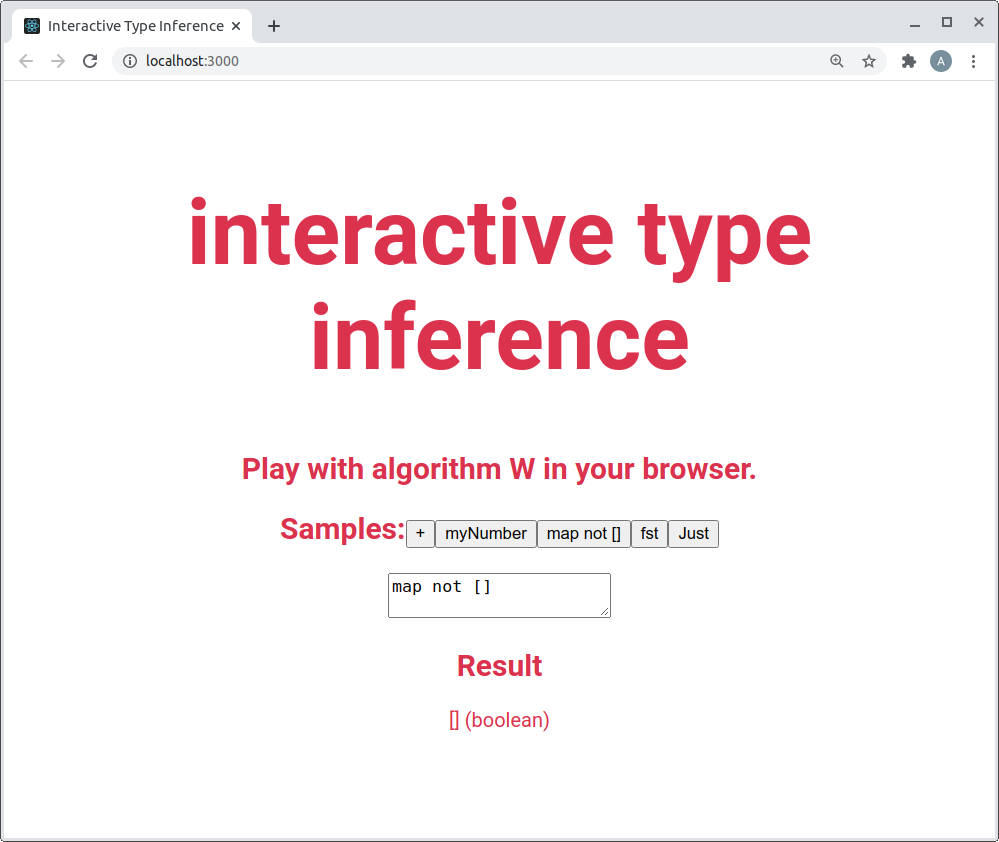
\includegraphics[width=1.023\linewidth]{images/image1.png}
  \caption{Tests for the algorithm-w library, using the custom toHaveType matcher}
\end{figure}

\subsection{Create the web application}\label{id:h.cwlbt58wsbeg}

Finally, the deliverable that users will directly interact with is the web application. This will allow them to enter an expression, and send it through the lexer, parser and type inference algorithm. The results will then be displayed back to the user, showing the steps the type inference algorithm took.

The web application itself is written in TypeScript, using the React framework. Using React helps with state management, should improve productivity and make testing considerably easier. Additionally, if the project is extended with more algorithms it will be possible to reuse components and be generally nicer to refactor.

\subsubsection{Extension}\label{id:h.hltng6i6eh9g}

Ideally, there would be time to test the application on real university students to try to determine whether it is an effective teaching aid. This would likely be showing them the application, explaining what it does and seeing how they use it, and testing whether they have a better understanding of type inference afterwards. Their feedback could be used to improve the application, and be valuable for the evaluation in the final report.

\subsubsection{Progress}\label{id:h.gmrcoirmlt2e}

A basic web application that accepts the language and displays the final result of the type inference algorithm has been developed. However, the language syntax is restricted, displaying the AST has not been implemented and the steps the algorithm has taken are not displayed. These limitations arise from the parser being incomplete and the algorithm W implementation not emitting steps yet.

{\centering \begin{figure}[h!]
  \centering
  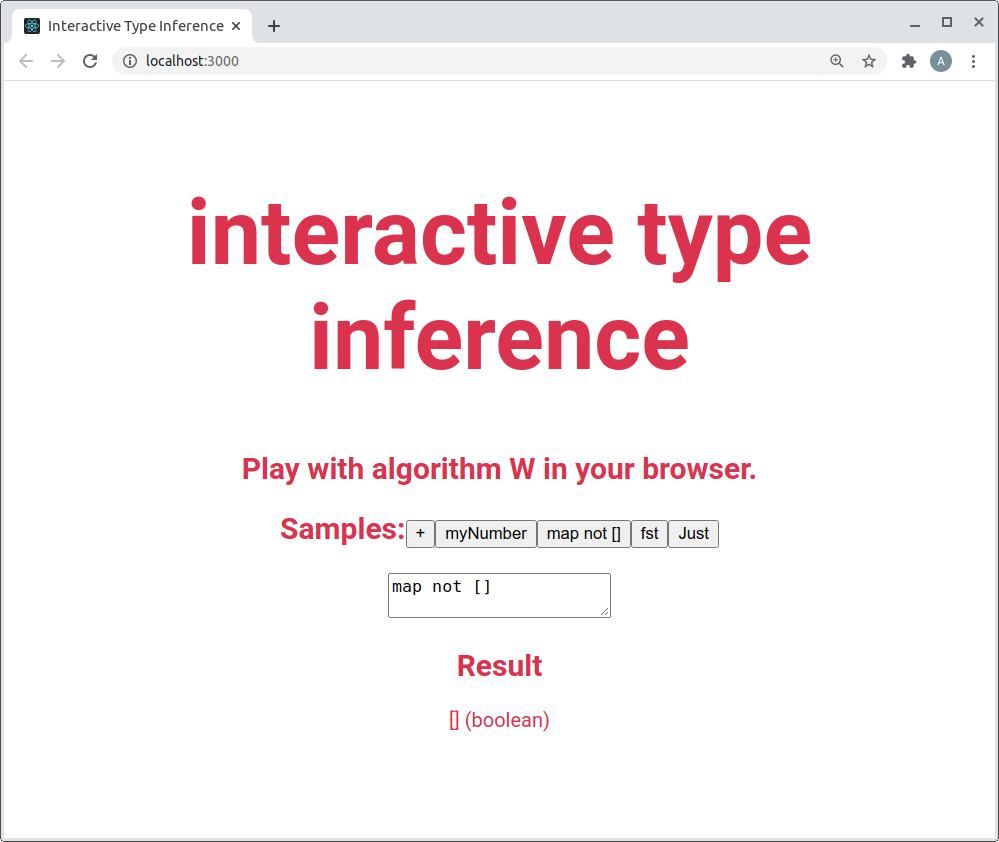
\includegraphics[width=0.837\linewidth]{images/image3.png}
  \caption{The web application showing the result of running algorithm W on an expression}
\end{figure} \par}

\section{Methods}\label{id:h.em0ria5zbf4p}

\subsection{Research process}\label{id:h.ew85fk610kqt}

I have maintained a list of resources and my notes on them. This will be invaluable for writing the final report’s background section, but also for referring back to refresh my memory of certain topics.

Additionally, this list contains a backlog of resources to explore. This ensures my research stays organised and I do not miss potentially important papers.

\subsection{Software development process}\label{id:h.d99ru3rx4zo}

Development is taking an agile approach, for three reasons: flexibility, early and frequent delivery and the individual nature of the project.

The approach must be flexible, as the project scope may well change as I get a better understanding of the area and gain user feedback. Additionally, one of the goals of the module is to be innovative and creative\cite{ref14} and so allowing for change over time provides the freedom to do this.

The approach should provide working software early and frequently, as for evaluation purposes it is better to have some kind of working software to show even if it lacks certain features, rather than only incomplete parts. Additionally, this allows for getting user feedback early, which combined with being flexible means the project can be adjusted to better serve user needs. Lastly, it will be easier for my supervisor to see the state of the software, and therefore be able to advise me on the project. This has been put into practice as I already have a functioning web application which accepts a basic expression and returns its type from a type inference algorithm.

As the project is an individual one, there is no coordination between developers necessary. This reduces the need to precisely plan and document how the components will integrate with each other, and the order components need to be delivered in. Therefore, waterfall or other heavily plan-based methods would not be beneficial over agile methods.

Automated unit, component and integration tests are written while developing the software. Good testing not only catches bugs, but enables confidence in making changes as they can be made while being sure the software still functions correctly. This supports the flexible agile software development approach. Tests can also act as proof that software requirements have been met, useful for my project supervisor and final evaluation.

\begin{figure}[h!]
  \centering
  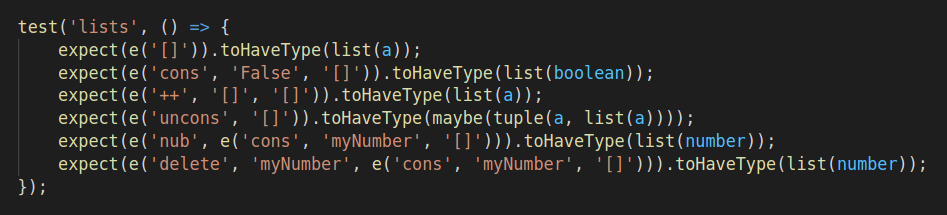
\includegraphics[width=1.023\linewidth]{images/image2.png}
  \caption{An automated test for the web application, which simulatenously tests many components of the system at once.}
\end{figure}

\subsection{Write-up process}\label{id:h.bhx39g801ds4}

The final report is the highest weighted assessment (80\%) of the project and therefore requires attention throughout.

I have been frequently updating my notes for the final report, adding points such as decisions taken and their reasons. Despite this, I expect writing and editing to take a significant amount of time at the end of the project.

\subsection{Communication and meetings}\label{id:h.k8ippxnoat7q}

Due to the ongoing COVID-19 pandemic, all communication and meetings will continue to take place online. Both my supervisor and I are used to using online communication tools and this has worked well so far, with the Tier 2 restrictions in Coventry and the national lockdown since the specification not having negatively affected communications.

I have had regular weekly meetings with my supervisor to keep them updated on the project and get help with any problems. The beginning and end of the project are likely to require the most guidance, as understanding existing resources on type systems was difficult, and reviewing the final report is likely to involve a lot of discussion.

In addition to these regular meetings, we sometimes chat on Slack and occasionally have other meetings including group meetings with other project tutees.

\section{Schedule}\label{id:h.7o2zxvygqpnu}

The schedule is an idea of how work might get done over time, but may change as the project goes on. My supervisor will be kept informed of major changes to this plan. Weeks start on Monday.

\subsection{Original schedule}\label{id:h.7j9eipb829lw}

Evaluating my progress against my original project specification, the project is ahead of schedule for building the lexer, parser and web application. Additionally, algorithm W was implemented ahead of schedule, but it has not yet been extended to report major steps taken.

\subsubsection{Term 1}\label{id:h.wrykjazjnc9}

Week 1: Flesh out the project aims and write an initial draft of the specification.

Week 2: Finish the specification and research deeper into the Hindley-Milner type system and lambda calculus.

Week 3: Focused reading on type systems and type inference algorithms, with particular attention to Hindley-Milner and algorithm W.

Week 4: Set up initial tooling (GitHub repos, TypeScript library structures, automated backups etc.) and start implementing algorithm W.

Week 5: Finish implementing a basic algorithm W.

Week 6: Finish algorithm W, including extending it to report major steps taken to be visualised later. Review all the associated code, tests, documentation, CI setups and report sections created since week 4.

Week 7: Focus on other modules’ coursework, including CS325 Compiler Design and CS342 Machine Learning and IB2B40 Digital Business in Modern Organisations.

Week 8: Write up the progress report.

Week 9: Create basic web application to start displaying steps of the type inference algorithm for some fixed example ASTs. This week I will also likely be busy with courseworks for CS342 Machine Learning, CS345 Sensor Networks and Mobile Data Communications and CS352 Project Management.

Week 10: Start work on creating a language specification, and developing a lexer and parser for it. When applied to an expression in the language, these will return an AST which to be consumed by the type inference algorithm.

Over the winter break, I’ll attempt to finish the lexer and parser.

\subsubsection{Term 2}\label{id:h.4jcij8mlihji}

Weeks 1-3: Ensuring the whole system works together, and finishing off anything incomplete. Once complete, work will begin on extensions such as implementing another type inference algorithm or user-testing.

Weeks 4: Critically evaluate the software so far, and whether it meets the objectives set out in this document, and any updated objectives as per Term 1’s progress report.

Weeks 5 and 6: Write up any missing draft sections of the final report.

Weeks 7 and 8: Prepare presentation.

Week 9/10: Deliver presentation and continue writing up the final report.

Over spring break, I’ll continue editing the final report alongside revising for summer exams.

\subsubsection{Term 3}\label{id:h.l1bn0snl39c1}

Week 1: Final touches on the final report.

Week 2: Submit final report.

\subsection{Revised schedule}\label{id:h.p9vfbpk6rnb6}

\subsubsection{Term 1}\label{id:h.p2x8af4pn3a5}

Week 9: Start extending algorithm W to report steps taken. This week I will also be busy with courseworks for CS345 Sensor Networks and Mobile Data Communications and CS352 Project Management. Additionally, disruption is likely as it may be the designated travel window for students for the winter break so I may be moving.

Week 10: Display the AST and steps taken in the web application. Start rewriting lexer and parser with a parser-combinator library to return an AST.

Over the winter break, I’ll attempt to finish the lexer and parser.

\subsubsection{Term 2}\label{id:h.5axy8qlqt2n8}

Weeks 1-3: Ensuring the whole system works together, and finishing off anything incomplete. Once complete, work will begin on extensions such as implementing another type inference algorithm or user-testing.

Weeks 4: Critically evaluate the software so far, and whether it meets the objectives set out in this document, and any updated objectives as per Term 1’s progress report.

Weeks 5 and 6: Write up any missing draft sections of the final report.

Weeks 7 and 8: Prepare presentation.

Week 9/10: Deliver presentation and continue writing up the final report.

Over spring break, I’ll continue editing the final report alongside revising for summer exams.

\subsubsection{Term 3}\label{id:h.jbcgtsb8n2zo}

Week 1: Final touches on the final report.

Week 2: Submit final report.

\section{Resources}\label{id:h.8b8ghk7r824a}

Git is being used for version control, as it is robust, well-used and I have experience with it. This allows rolling back to previous working versions of the software if necessary, and acts as a change log of how the project has evolved. Also, it makes diffing versions of the code easy, so my supervisor can easily determine what has changed since last view. Git is free software.

GitHub is being used for git hosting, which allows me to easily sync changes between machines, and allows sharing the code with my supervisor easily. GitHub offers these features for free.

GitHub also acts as an external backup of the code. This ensures my work would not be lost if my personal computer was. However, a bad force push could theoretically cause data loss, so at major milestones I have stored snapshots of the code on Google Cloud Platform (avoiding Azure to maximise resiliency, as GitHub runs on Azure). This is within the free tier limits.

In my project specification, GitHub was considered for project, issue and pull request management. However after evaluating the project needs this was found to be unnecessary. As a single developer I am able to understand the overall structure of the code having written it, and a simple notepad has sufficed for task tracking.

GitHub Actions provides continuous integration, providing build and test failure visibility on each commit. In future, continuous deployment will ensure the live application is kept up to date with any changes, making it easy to manually test and for my supervisor to see the current state of the system. GitHub Actions is free on public repositories, and offers 3000 free build minutes a month and 1GB of storage on private repositories. Having reviewed my billed usage, I fall well under this limit.

Most of the system is written in TypeScript, a programming language developed by Microsoft, for reasons explained in the objectives section. Its compiler is freely available.

VS Code is being used to write TypeScript, as it is the most popular code editor for it and is well designed for it. Additionally, I have used VS code in the past, and it can be used to write the Latex sources for the reports. VS Code and its TypeScript extension are free.

By the end of term 1, the web application will be available at all times to manually test and for my supervisor to see. Using a cloud platform will allow for this without having to maintain hardware. Exactly which cloud hosting provider used will be chosen later, but I expect this to be free or low cost.

My supervisor and I chat on Slack, making communication easy and efficient. For our regular meetings we have been using Microsoft Teams.

Draft reports have been written in Google Docs, as it is easy to use, version-controlled and offers good reviewing features. At major milestones this is synced with the git repository, so is included in the git backup on GitHub and Google Cloud Platform. For more control over typesetting, the tool gdoc2latex\cite{ref15} was developed to convert a Google Docs document to a LaTeX document. GitHub actions automatically uses this tool to keep the Google Docs and LaTeX versions in sync within the repository.

\section{Risk review}\label{id:h.lkcg9956g3l}

\begin{center}\begin{tabular}{ |l|l|l| }
  \hline
  \textbf{Description} & \textbf{Likelihood} & \textbf{Severity} \\
  \hline
  Illness or other circumstances affecting me & Medium & High \\
  \hline
  Illness or other circumstances affecting my supervisor & Medium & Medium \\
  \hline
  Project activities take more time than expected & Medium & High \\
  \hline
  Other activities take more time than expected & High & Medium \\
  \hline
  Temporary internet or development machine unavailability & Low & High \\
  \hline
  Loss of data on own machine, GitHub or Google Docs & Low & Low \\
  \hline
  Loss of data and all backups & Very low & Very high \\
  \hline
  Temporary GitHub unavailability & Medium & Very low \\
  \hline
  Permanent GitHub unavailability & Very low & Low \\
  \hline
  Temporary Slack unavailability & Medium & Low \\
  \hline
  Permanent Slack unavailability & Very low & Very low \\
  \hline
  Temporary Google Docs unavailability & Low & Low \\
  \hline
  Permanent Google Docs unavailability & Very low & Low \\
  \hline
  Temporary cloud hosting service unavailability & Low & Low \\
  \hline
  Unexpected financial costs for cloud services & Low & Low \\
  \hline
\end{tabular}\end{center}

In the project specification, careful attention was paid to identifying and mitigating risks. Since then, the risks have not changed significantly and I believe these residual risks remain acceptable. The greatest risks are still unforeseen circumstances or general overrunning which are beyond my control. To mitigate their impact there is still some slack in the project schedule for extensions, and taking a flexible agile approach may help adjusting the project scope to accomodate for necessary changes.

I will continue monitoring the project and notify my supervisor if I identify any potential risks, or if an identified risk has changed likelihood or severity.

\section{Ethical and safety review}\label{id:h.yity1y53zkk0}

Since the project specification, no additional ethical or safety concerns have arisen.

As noted in the specification, user-testing may be carried out with students and other academics to get their feedback on the web application. This will not involve deception, coercion or involve vulnerable groups so does not require ethical review by the University’s Biomedical and Scientific Research Ethics Committee. Data will only be collected and held with the subject's informed, unambiguous consent.

This project continues not to have any serious health and safety implications. HSE guidelines will continue being followed for the use of display screen equipment and any activities will be carried out in line with government COVID advice.

I will continue looking out for ethical or safety issues and notify my supervisor if I have any potential concerns.

\bibliography{index}

\bibliographystyle{abbrvurl}

\end{document}